% THIS IS SIGPROC-SP.TEX - VERSION 3.1
\documentclass{sig-alternate}

% Additional packages
\usepackage{graphicx}
\usepackage{color}
\usepackage{url}
\usepackage{algorithm}
\usepackage[noend]{algpseudocode}
\usepackage{amsmath}
%\usepackage{amsthm}
\usepackage{amsfonts}
\usepackage{amssymb}
\usepackage{booktabs}
\usepackage{multirow}
\usepackage{ifpdf}
% Custom commands
\usepackage{custom_commands}

%\newcommand{\note}[1]{\relax} %{\color{red}#1}}
\newcommand{\note}[1]{{\color{red}#1}}

\newcommand{\prg}[1]{\paragraph{#1}}
%\newcommand{\prg}[1]{\textbf{#1}}

\newcommand{\Siren}{\textsc{Siren}}
\newcommand{\ReReMi}{\textsc{ReReMi}}

\begin{document}
\special{papersize=8.5in,11in}
\setlength{\pdfpageheight}{11in}%{\paperheight}
\setlength{\pdfpagewidth}{8.5in}%{\paperwidth}


\title{Siren: An Interactive Tool for Mining Geospatial Redescriptions}
\subtitle{[Demo]}

\numberofauthors{2} 
\author{
% 1st. author
\alignauthor
Esther Galbrun\\
       \affaddr{Department of Computer Science}\\
       \affaddr{University of Helsinki, Finland}\\
       \email{galbrun@cs.helsinki.fi}
% 2nd. author
\alignauthor
Pauli Miettinen\\
       \affaddr{Max Plack Institute for Informatics}\\
       \affaddr{Saarbr{\"u}cken, Germany}\\
       \email{pmiettin@mpi-inf.mpg.de}
}

\maketitle
\begin{abstract}
  We present \Siren, an interactive tool for mining geospatial
  redescriptions.  Redescription mining is a powerful data analysis
  tool that aims at finding alternative descriptions the same
  entities.  For example, in biology, an important task is to identify
  the bioclimatic constraints that allow some species to survive, that
  is, to describe geographical regions in terms of both their
  bioclimatic conditions and the fauna that inhabits them.  When the
  entities are geographic locations, we qualify the redescriptions as
  geospatial.  
  
Using \Siren, a user can explore geospatial data of his
  interest by visualizing the redescriptions on a map, interactively
  edit, extend and filter them\footnote{More details about \Siren's
    features, additional snapshots and a demonstration video are available online at
    \url{http://www.cs.helsinki.fi/u/galbrun/redescriptors/siren/}.}.

  We will demonstrate the use of the \Siren\ system on two applications:
  niche-finding over Europe and the exploration census statistics and
  electoral campaign funding of counties of the United-States.
\end{abstract}

\category{H.2.8}{Information Systems}{Database Applications}[Data Mining]
\category{H.5.2}{Information Interfaces and Presentation}{User Interfaces}

\terms{Redescription Mining, Geospatial data, Application}

%\keywords{ACM proceedings, \LaTeX, text tagging} % NOT required for Proceedings

\section{Introduction}
%\subsubsection{Redescription Mining}
Finding multiple ways to characterize the same entities is a problem
that appears in many areas of science.  In medical sciences, one might
want to find a subset of patients sharing similar symptoms and similar
genes. Describing geographical regions in terms of both their
bioclimatic conditions and the fauna that inhabits them is a second
example instance. This is a task of great importance for biologists.
 A very
simple example of a redescription in this setting could say that
areas where polar bears live are areas where March's mean temperature
is between $-16$ and $-11$ degrees Celsius and May's mean temperature
is between $-3$ and $-7$ degrees Celsius.

However, in general, to find such alternative descriptions of the data one would
need to determine by hand the query on one side before
looking for the best matching query on the other side, using some type
of classification. This typically prevents queries involving more than
one variable to be tested.  \emph{Redescription Mining} aims at
solving this tedious task by automatically identifying the best
redescriptions.

More formally, given data containing entities with two sets of characterizing
variables. The task is to find a pair of queries, one query for both
sets of variables, such that both queries describe (almost) the same
set of entities.

%\note{Two views of redescription mining}
The results of redescription mining, the redescriptions, can be
approached from two points of view. On one hand, we can study the
variables and conditions appearing in the queries, providing
valuable information about these variables. On the other hand, we can
study the support set of the redescriptions, i.e.\ the subset of
entities where both queries of a redescription hold. When the data
is geospatial, that is, the entities are connected to geographical locations, the
latter approach becomes even more important. A meaningful geospatial
redescription should define coherent areas using expressive
queries. The goal of \Siren\ is to facilitate the analysis of the
redescriptions using both of the approaches simultaneously.

% \begin{figure}[hb]
%   \centering
% \includegraphics[width=.5\textwidth]{screenshots/siren_map.png}
%   \caption{Map panel, displaying a redescription on a map.}
%   \label{fig:map_panel}
% \end{figure}

\begin{figure*}[t]
  \centering
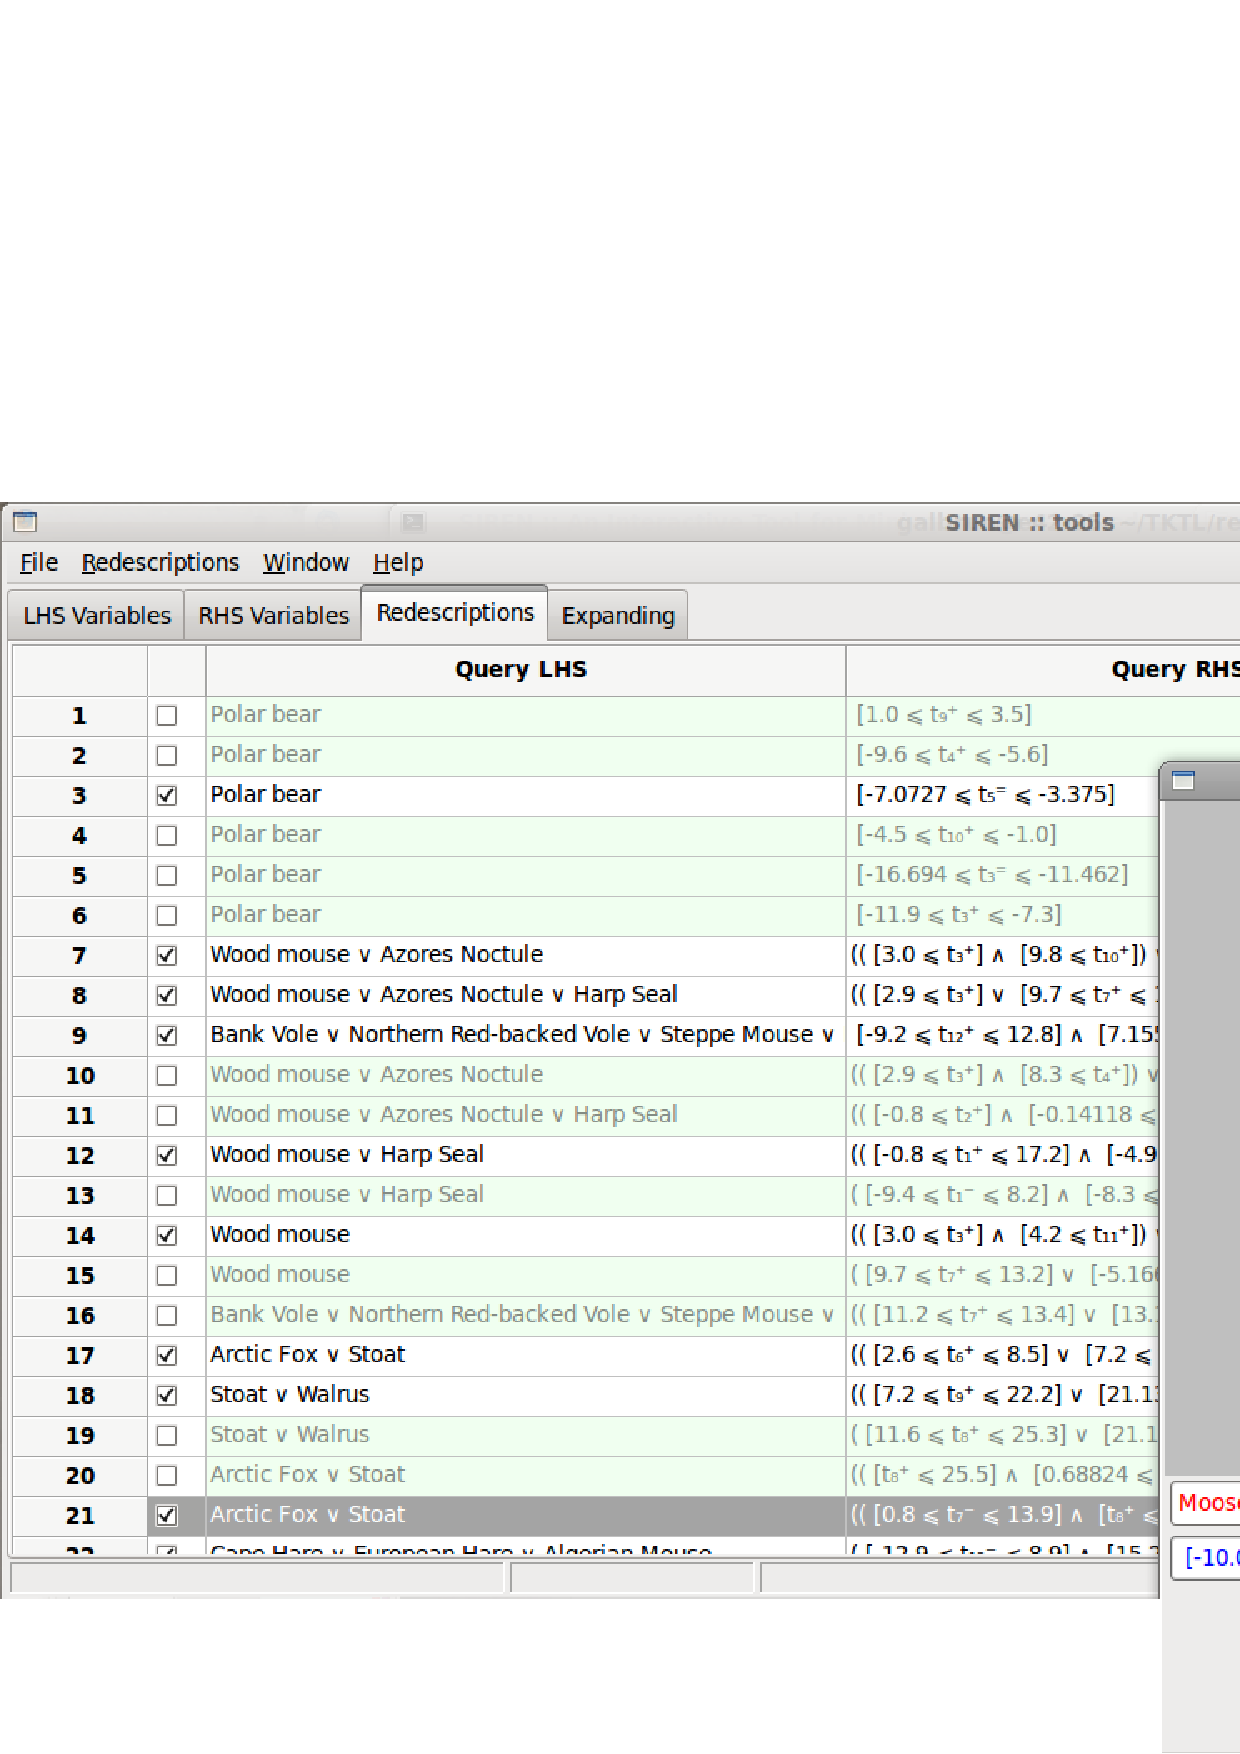
\includegraphics[width=\textwidth]{screenshots/both_panels_02.png}
  \caption{The \Siren\ interactive mining tool. The panel in the background displays a list of mined redescriptions. The foreground panel contains a plot of a selected redescription on a map, allowing edition and providing updated quality indicators.}
  \label{fig:both_panels}
\end{figure*}

Redescription mining aims at simultaneously finding multiple
descriptions of a subset of entities which is not previously
specified.  This is in constrast with other methods like Emerging
Patterns Mining (EPM), Contrast Set Mining (CSM) or Subgroup Discovery
(SD) (see \cite{kralj09supervised} for a unifying survey) or general
classification methods, where target subsets of entities are specified
via labels.  Currently, redescription mining is a purely descriptive
approach, its predictive power remains to be explored.  Since its
introduction in~\cite{ramakrishnan04turning} various algorithms have
been proposed for Boolean redescription mining, based on approaches
including decision
trees~\cite{ramakrishnan04turning,kumar07redescription},
co-clusters~\cite{parida05redescription}, and frequent
itemsets~\cite{gallo08finding}.  At the core of \Siren\ is
\ReReMi~\cite{galbrun11black}, a greedy algorithm that extends
redescription mining to categorical and numerical variables.

\section{Use-case scenario}
\label{sec:scenarios}
We exemplify the use \Siren\ by going through a typical workflow of
mining geospatial redescriptions.  A snapshot of the system
displaying a list of redescriptions with one
selected redescription plotted on a map is shown in
Fig.~\ref{fig:both_panels}.

\prg{Initial redescription mining}
Given the data, a natural first step is to use a redescription mining
algorithm to find the initial set of redescriptions. 

When the initial set of redescriptions is mined, the user can study the
interesting redescriptions plotted on a map.
Uninteresting redescriptions can be manually disactivated.
 
\prg{Editing a redescription} 
The interaction with \Siren\ start after the initial set of
redescriptions is mined, as it allows the user to visualize, edit,
filter and refine the redescriptions.  It is typical that the
algorithm returns redescriptions that the user wants to edit. For
example, some redescriptions might be overly complex, or have
exceedingly accurate boundaries for numerical variables. The user can
easily select the redescription he wants to modify, open it in a map
window and start editing it. \Siren\ updates the map and important
statistics (accuracy, $p$-value, etc.) about the redescription,
allowing the user to see the effects of his edits immediately. This
makes it easy for the user to check, e.g.\ whether the simplified
redescription would still be acceptably accurate.


\prg{Extending a redescription}
Sometimes the user wants to focus only on one of the queries in the
redescription, on some particular variable of interest or on part of an existing redescription. 
\Siren\ allows the user to automatically extend a given
redescription, i.e.\ let the algorithm add new items to the queries to
make the redescription as accurate as possible.
% (see Fig.~\ref{fig:extending}). 

The extension mechanism of \Siren\ is based on the beam search implemented in
the \ReReMi\ algorithm.  It can also be used to explore more specific
alternative extensions to a redescription, that the beam search might
have discarded at some point of the search because they were not the
best extensions.


% \begin{figure*}
%   \centering
% 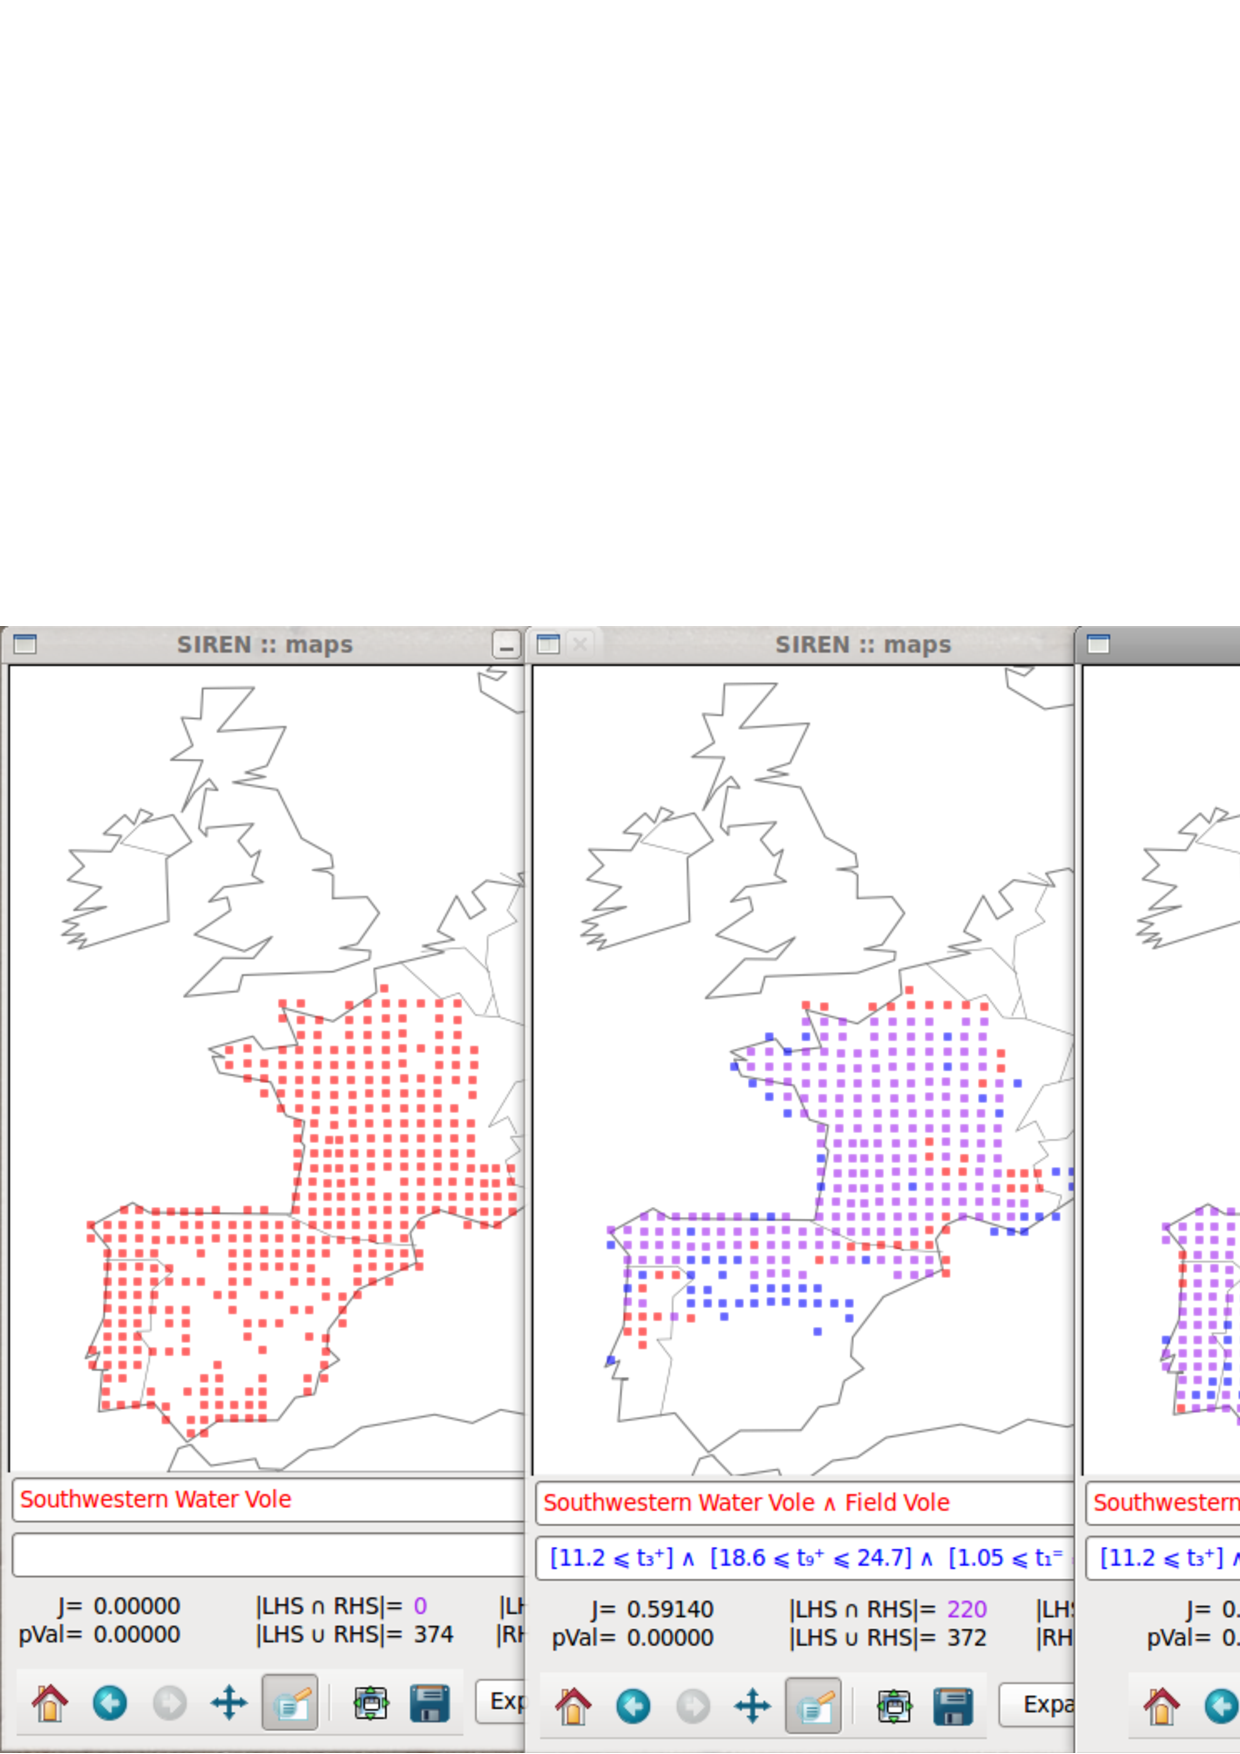
\includegraphics[width=\textwidth]{screenshots/comparison.png}
%   \caption{Map panels, comparing redescriptions.}
%   \label{fig:comparison}
% \end{figure*}



\prg{Using subsets of variables}
Finally, many times a set of redescriptions contain the same pair of
variables. This can happen, e.g.\ when these two variables are highly
correlated. The user, however, might want to see redescriptions that have
only one of these variables, not both. \Siren\ makes this simple: the user
only has to select a redescription, remove the variable he does not
want to have from the redescription, unselect it from the list of variables, and
extend the redescription. \Siren\ will not use the unselected
variables when extending or mining redescriptions.


% \begin{figure}
%   \centering
% \includegraphics[width=.5\textwidth]{screenshots/variables_05.png}
%   \caption{Tool panel, uselecting variables.}
%   \label{fig:map_panel}
% \end{figure}

% \begin{figure}
%   \centering
% 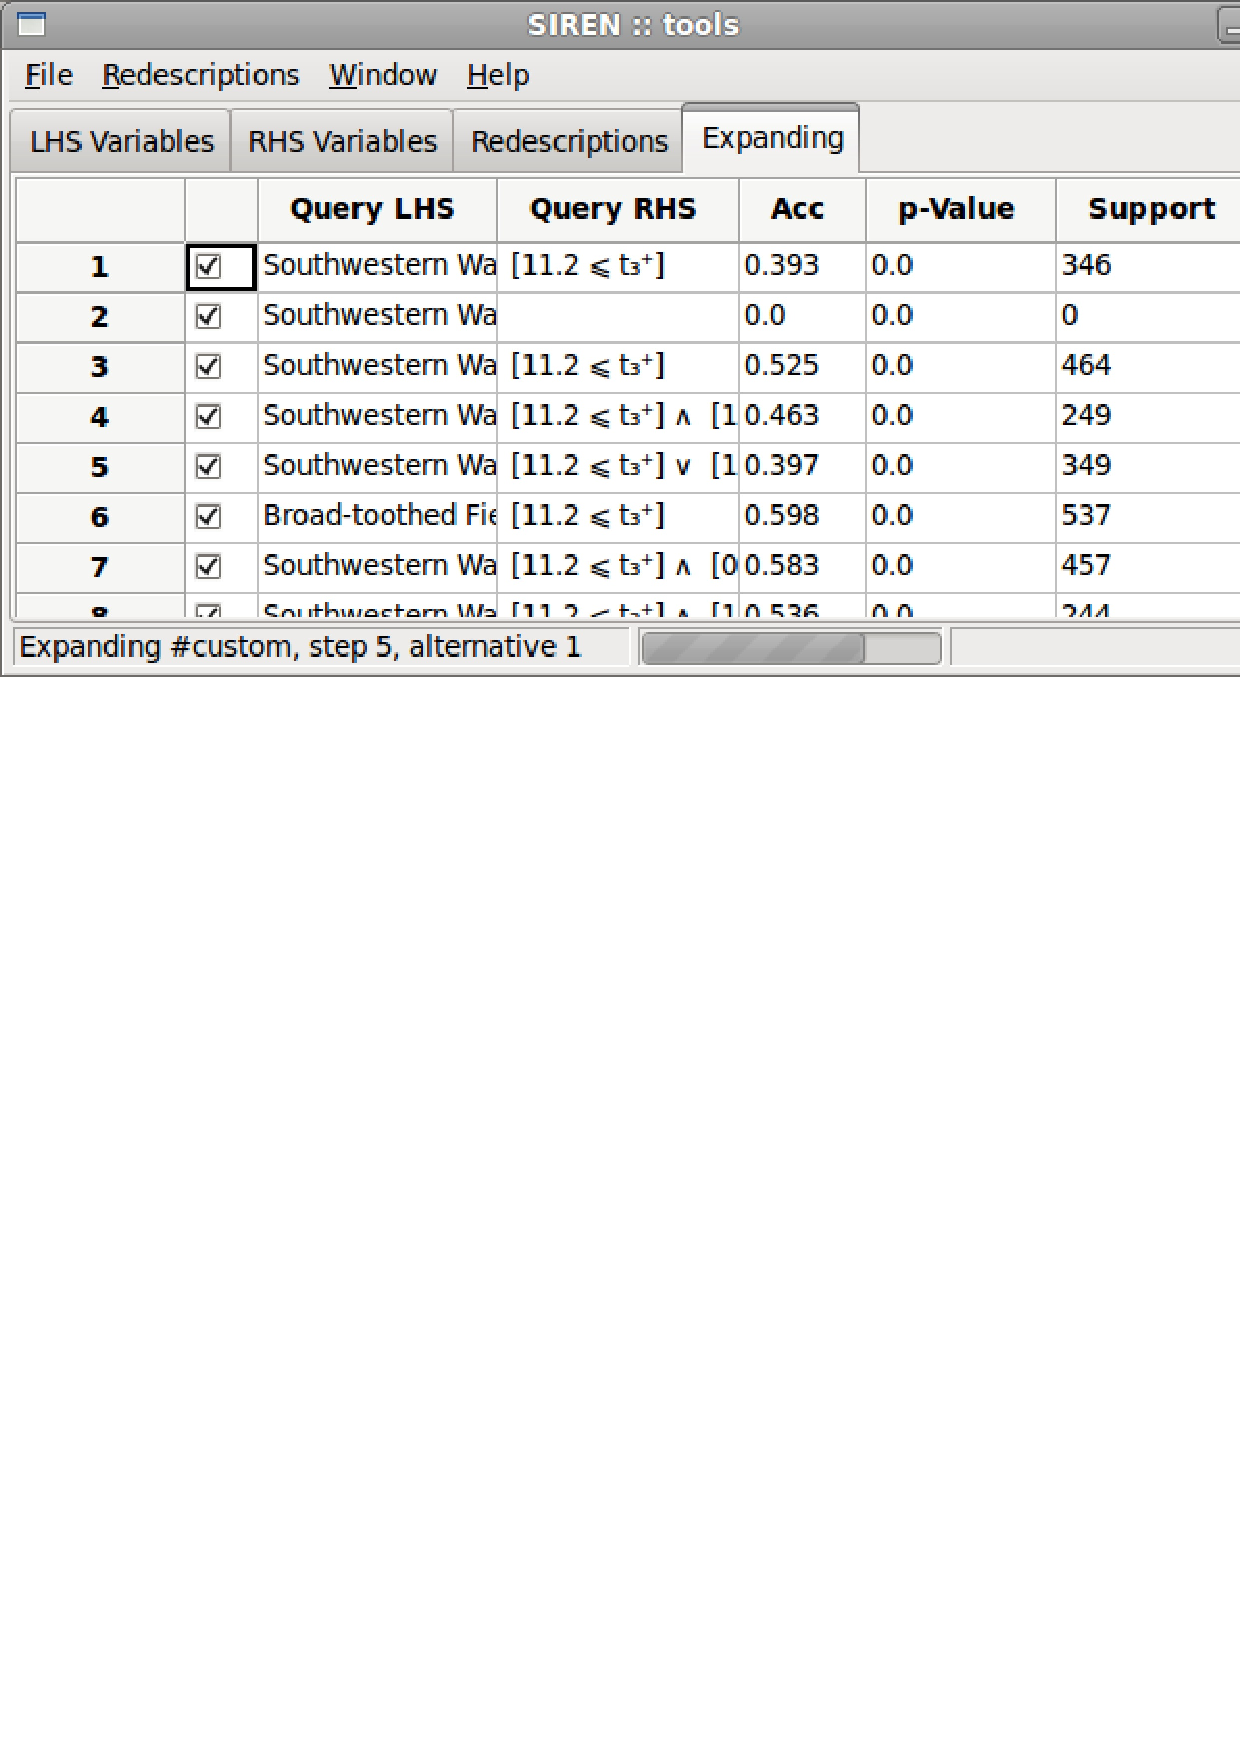
\includegraphics[width=0.5\textwidth]{screenshots/extending.png}
%   \caption{Tool panel, extending a redescription.}
%   \label{fig:extending}
% \end{figure}



\prg{Filtering redundant redescriptions}
\label{sec:filt-redund-redescr}
It is common to see a set of redescriptions that cover approximately
the same area even if they have (somewhat) different set of
variables. In such cases it is important to be able to recognise and
remove redundant redescriptions, i.e.\ redescriptions that do not
convey significant new information, lest the user be overwhelmed with
the number of found redescriptions. Again, \Siren\ allows automatic
filtering of redundant redescriptions. The user can either select a
redescription and ask \Siren\ to filter out all redescriptions that
are redundant with respect to the selected one, or \Siren\
can go throught the whole list of redescriptions filtering out all
redescriptions that are redundant with respect to some
earlier-encountered (i.e.\ better) redescription. Naturally the user
can revert the decisions made by \Siren\ whenever he wants to.


% \begin{figure}
%   \centering
% \includegraphics[width=.5\textwidth]{screenshots/redescriptions.png}
%   \caption{Tool panel, filtering redescriptions.}
%   \label{fig:filtering}
% \end{figure}

\prg{Outputting the results}
\label{sec:outputting-results}
Finally, \Siren\ facilitates the distribution of the results:
redescriptions can be exported in easy-to-read format and the
maps associated to redescriptions can be easily converted to
publication-ready files. 

\section{Sample applications}
We will demonstrate the application of \Siren\ in two different domains. 

\prg{Biological niche-finding}
An important problem in biology, known as \emph{niche-finding} is a
particular instance of redescription mining.  The bioclimatic
constraints that must be met for a certain species to survive
constitute that species' bioclimatic envelope, or niche~\cite{grinnell17niche}.  Finding such
envelopes can help, e.g.\ to predict the results of global
warming~\cite{pearson03predicting}.  A number of methods, involving
regression, neural networks, and genetic algorithms
(see~\cite{soberon05interpretation}) have been developped over the
past ten year to model the bioclimatic envelope.
\textsc{BIOMOD}~\cite{thuiller09biomod} being a good example of
a modelling tool used this domain.  But to the best of our
knowledge, none of these methods allows automatically finding both the
set of species and their envelope.

We demonstrate the application of \Siren\ on this task using data
that describes spatial areas of Europe, squares of side roughly 50
km$^2$.  The left hand side data contains information about the
mammals that live in these areas, while the right hand side consists
of bioclimatic variables. The data comes from two publicly available
datasets: European mammal atlas~\cite{mitchell-jones99atlas} and
Worldclim climate data~\cite{hijmans05very}.

\prg{US counties statistics}

% \begin{figure}
%   \centering
% \includegraphics[width=.5\textwidth]{screenshots/siren_map_us_00.jpg}
%   \caption{Map panel, displaying a redescription on a map.}
%   \label{fig:map_panel}
% \end{figure}

To demonstrate the flexibility of the \Siren\ mining tool, we illustrate its usage on
a dataset from an entirely different domain, describing the counties
of continental United-States.  This time, the left hand side data
contains socio-economic indicators about the counties, such as
population, age distribution or educational attainment. The right hand
side consists of data about funding of the electoral campaigns in
2006, 2008 and 2010. The data has been gathered from two public
websites: FedStats\footnote{http://www.fedstats.gov/} and Open
Secrets\footnote{http://www.opensecrets.org/elections/}.

\section{Technical details}
\Siren\ is based on the \ReReMi\ redescription mining
algorithm. This greedy algorithm uses an
efficient on-the-fly discretization technique to extend redescription
mining to categorical and numerical variables.
We now give an outline of the concepts and algorithms involved in mining redescription, more details can be found in the original publication~\cite{galbrun11black}. 

The input data consists of a set of entities $E$ with two set of
characterizing variables, $V_\iLHS$ and $V_\iRHS$.  Each variable $v$
corresponds to a column vector containing the values taken by all the
entities.  We consider three types of variables: Boolean, categorical,
and numerical (real-valued).  If $v\in V$ is Boolean, we interpret the
column corresponding to it as a truth value assignment in a natural
way.  If $v\in V$ is real-valued, we consider an interval $[a, b]$,
and the truth value assignment induced by the relation
$v\in[a,b]$. Finally, if $v$ is categorical, we consider the relation
$v=c$, where $c$ is some category.  These truth assignments and their
negations constitute \emph{literals} which can be combined using the
Boolean operators $\land$ (and) and $\lor$ (or) to form
\emph{queries}.  Then, a redescription is simply a pair of queries
over variables in $V_\iLHS$ and $V_\iRHS$ respectively, denoted as
$R=(q_\iLHS,q_\iRHS)$.
The support of a query is the subset of entities for which the query holds true.
The \emph{accuracy} of a redescription $R=(q_\iLHS,q_\iRHS)$ is 
measured using the \emph{Jaccard coefficient} 
\[
\jacc(R)= \jacc(q_\iLHS,q_\iRHS) = \frac{\abs{\supp(q_\iLHS,q_\iRHS)}}%
{\abs{\supp(q_\iLHS)\cup\supp(q_\iRHS)}}.
\]

The search space of all Boolean formulae is too huge to be manageable.
Therefore, we need to restrict ourselves to a subset of formulae that
provides a good compromise between expressive power, difficulty of the
search, and interpretability.
For this purpose, we consider queries that can be parsed in linear
order, without trees, and allow every variable to appear only once.
For example, $(a \lor b) \land \lnot c$ is an acceptable query, but
$(a \land b) \lor (c \land d)$ is not. Yet, the search space remains
exponential and we still resort to a heuristic pruning during the
search.  We use a strategy similar to beam-search to explore the
solution space.  The basic idea is to construct queries bottom-up,
starting from singleton redescriptions (i.e.\ both queries contain
only one literal) and progressively extending them by appending
operators and literals.  For example, we could start with a pair $(a,
\lnot b)$, and try to extend it to $(a\land c, \lnot b)$, $(a \lor c,
\lnot b)$, $(a \land \lnot c, \lnot b)$, etc. After evaluating all
possible one-step extensions, we select the best candidates and extend
them in turn. This process requires a book-keeping procedure to avoid
repeatedly generating the same queries.  When no new redescription can
be generated, we move to the next initial pair.  

We exploit some
simple observations to make the computation of accuracy more
efficient. This allows to evaluate candidates faster, especially
extensions with non-Boolean variables.
We compute a \pValue{} that represents the probability that two random
queries with marginal probabilities (i.e.\ the fraction of entities
supporting them) equal to those of $q_\iLHS$ and $q_\iRHS$ have an
intersection equal to or larger than $\abs{\supp(q_\iLHS,
  q_\iRHS)}$. This probability uses the binomial distribution. The higher the
\pValue, the more likely it is to observe such a support for
independent queries, and the less significant the query. Redescriptions with too high \pValue{} can be discarded.

The formulation of redescription mining presented here assumes that the
describing variables are partitioned into two sets, $V_\iLHS$ and
$V_\iRHS$, and looks for a pairs of queries over these two sets,
respectively.  However, this can be naturally adapted to settings with
a single set of describing variables.  One might then search for pairs
of queries, with the constraint that the two subsets of variables
appearing in the queries of any redescription be disjoint or enable
the user to interactively determine the split between the variables.

\Siren\ and \ReReMi\ are implemented in Python.  The interface is built
with the \texttt{wxPython} Open Source GUI toolkit, ensuring
cross-platform compatibility.  The \texttt{matplotlib} library enables
to generate high quality figures seamlessly integrated in the
interface.  \Siren\ can handle any data provided in a compatible
format.

\section{Conclusions}
We present \Siren, a tool for interactively mining geospatial
redescriptions. It allows users to mine, vizualise, edit and extend
redescriptions.
We will give the chance to the public to experiment with \Siren\ and
together consider how this tool could be used to explore their own geospatial
data and help answer their data analysis need.

\bibliographystyle{abbrv}
%\nocite{*}
\bibliography{bibsiren}  
\balancecolumns

% That's all folks!
\end{document}

%%% Local Variables: 
%%% mode: latex
%%% TeX-master: t
%%% End: 
